\section{Annotation and corpus}

Annotating tweets have been one of the most difficult tasks. In their proposed model, Alvaro et al.~\cite{alvaro2015crowdsourcing} annotated over 1548 tweets in three categories: “First-class experience”, “Tweet written in English language”, and “Tweet about the drug”. There curated corpus is available~\footnote{\url{http://github.com/nestoralvaro/JBI_Pharmacovigilance}}. The ADR expert guideline is available as well~\footnote{\url{https://ars.els-cdn.com/content/image/1-s2.0-S1532046415002415-mmc1.pdf}}.

Sarker et al.~\cite{sarker2016social} in their follow-up work, proposed a corpus  of  267215  Twitter  posts  containing  at least one drug related keyword~\cite{sarker2017corpus}. They collected this data  over a four-month  period - from  November, 2014  to  February, 2015. This data contain over 250 medication related keywords. This data is available in their website~\footnote{\url{http://diego.asu.edu/Publications/Drugchatter.html}}. Alvaro et al.~\cite{alvaro2017twimed} presented a corpus of pharmacovigilance which compromised of 1000 tweets and 1000 PubMed sentences. For the task, they collected 165489 tweets and 29435 PubMed sentences. Their TwiMed pipeline annotation is shown in the Figure~\ref{fig:architecture-twimed-alvaro}.


\begin{figure}[h]
	\centering
	\begin{minipage}{0.45\textwidth}
		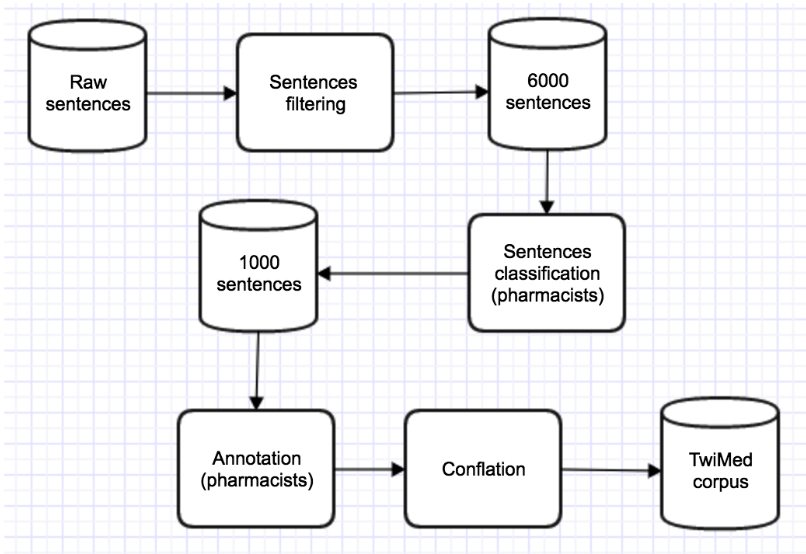
\includegraphics[width=0.99\linewidth]{Figures/b.png}
		\caption{TwiMed annotation pipeline by Alvaro et al.~\cite{alvaro2017twimed}.}
		\label{fig:architecture-twimed-alvaro}
	\end{minipage}
	\hfill
	\begin{minipage}{0.45\textwidth}
		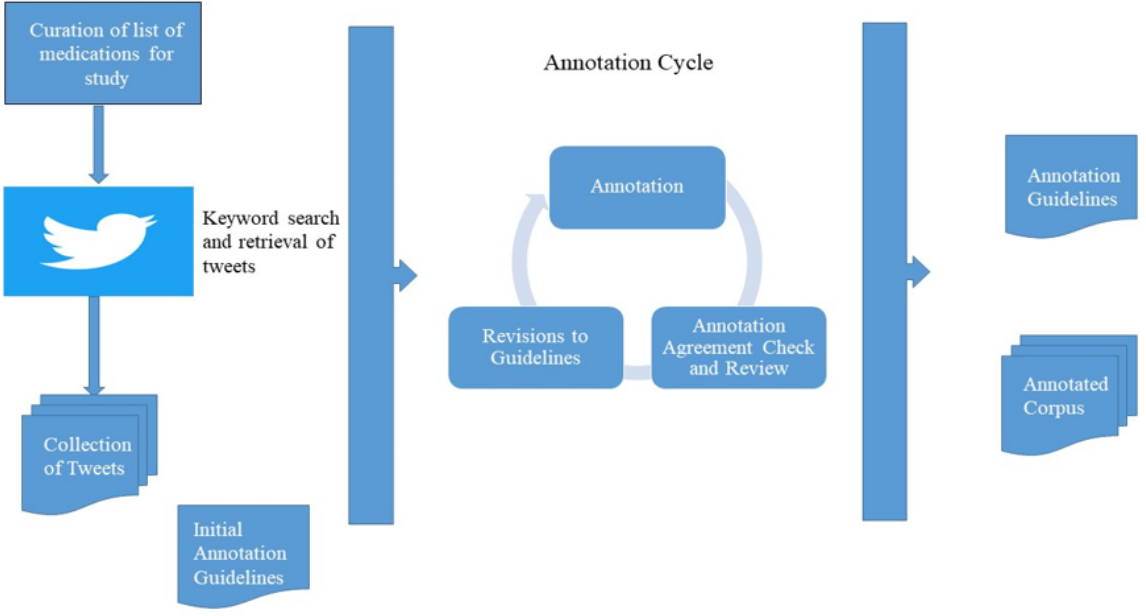
\includegraphics[width=0.99\linewidth]{Figures/d.png}
		\caption{Overview of the creation of the annotation guideline by O’Connor et al.~\cite{o2020promoting}.}
		\label{fig:annotation-oconnor}
	\end{minipage}
\end{figure}


Klein et al.~\cite{klein2017detecting} focused their study not only on detecting medications but also on distinguishing tweets whether they indicate the user possibly took it or merely mention medication. For this research, they annotated 10260 tweets. The annotation guidelines and a sample of the annotated data are available~\footnote{\url{https://healthlanguageprocessing.org/twitter-med-intake/}}. Later, Klein et al.~\cite{klein2019analysis} proposed a corpus of 27941 tweets for medication intake classification. They annotated them in three categories - “intake”, “possible intake”, and “no intake”. O’Connor et al.~\cite{o2020promoting} proposed an annotation guideline when they annotated 16443 tweets mentioning at least 20 abuse-prone medications. The guideline process is shown in Figure~\ref{fig:annotation-oconnor}. They categorized tweets into four categories: “potential abuse or misuse”, “non-abuse consumption”, “drug mention only”, and “unrelated”. The annotation guideline is available~\footnote{\url{https://tinyurl.com/y2zetam9}}.